\chapter{Discussion}
\label{ch:discussion}

\section{Summary of findings}

In the previous three chapters, I presented acoustic data from the vowels of 54 speakers of Cowlitz County, Washington. Chapter \ref{ch:elsewhere_shift}, which discusses the front lax vowels before obstruents, showed evidence for the Elsewhere Shift in this community. \bat has been in motion since at least the 1930s and shows signs of slowing down; among the women, \bet began shifting with the Baby Boomers and appears to have stopped with the Millennials, \bit exhibited an on-again-off-again pattern that suggests perhaps the tail end of one shift followed by the beginning of retraction as part of the Elsewhere Shift. The timing of these changes suggests a pull chain, but the direction of shifting was more similar to the parallel shifts found in Canada. Women shifted their vowels the most as far as relative position in the F1-F2 space is concerned, though both sexes changed the shape of the vowels' trajectories in tandem. The biggest difference between Cowlitz County speakers and Californians is that \bat was primarily lowered rather than retracted. The use of GAMMs helped discover that the first half of the trajectory changes more than the second half in apparent time.

Chapter \ref{ch:prenasal} presented acoustic data from the same front lax vowels but before nasals. The prenasal split was evident in \trap: while \bat was lowering in all groups, \ban was raising, with the exception of the women in Generation X who lowered it. For \ben and \bin, the women had the most change, but it was mostly in parallel with \bet and \bit, respectively. The men did not shift their vowels nearly as much in the F1-F2 space. Both sexes gradually diphthongized the vowels and changed their trajectories from C-shapes to something quite a bit more ``pointy.'' The Millennials were the ones who shifted the most relative to the other generations, and this was especially true for women and with \bang and \bing. There was not enough data for a full analysis of \beng, but preliminary findings suggest that it is similar to \bang.

In chapter \ref{ch:low_back}, I presented data on the low back vowels. I first demonstrated that the two vowels were not fully merged;  \thought has a more diphthongal trajectory and is higher and backer than \lot. When looking at the two vowels individually, there was relatively little change in apparent time in F1 or F2 for men or women for either vowel. The remarkable stability in this near-merger suggests that the bulk of language change happened before the oldest speakers in this sample were born, antedating \bat-lowering. I conclude that the approximation of these two low back vowels was the trigger that set the front lax vowels into motion.

The previous three chapters focused exclusively on formant measurements extracted from these speaker's speech. The patterns illuminated several clear trends in apparent time with respect to the Elsewhere Shift in Cowlitz County, namely that Millennial-aged participants used variants like those found in places like Oregon and California. Those chapters provided evidence to suggest that the Elsewhere Shift has spread into Washington. However, quantitative data can only say so much, and in this case, it is unclear how and why this shift is found in Cowlitz County but not in other areas of Washington. Fortunately, in addition to the acoustic measurements taken from these people's speech, the content of their interviews provides useful information that shed some light on the beginning of the Elsewhere Shift in this community.

This chapter deals exclusively on qualitative data gathered in these interviews and how these people's attitudes towards particular topics correlate with changes found in their speech. As mentioned in Chapter \ref{ch:methodology}, I entered the interviews with a set of questions that was tailored to speakers in this community, specifically addressing topics such as the Pacific Northwest, Longview and the surrounding areas, Portland and Seattle, and the logging industry. The responses to these questions varied significantly, but their polarity appeared to be correlated with age. Specifically, older people enjoyed Longview and were nostalgic about the ``good ol' days'' while younger people were less fond of their hometown and embraced Portland's ``weirdness'' culture. I hypothesize that this age division plays a major role in the linguistic patterns found among these people.

In this chapter, I present qualitative evidence to suggest that the shift in cultural views of Longview and Cowlitz County correlated with the changes in the timber industry that occurred in the late 1970s and early 1980s (see \S\ref{sec:rise_and_fall}). Specifically, I look at how Longview and views about Portland have changed over the years. In \S \ref{sec:trajs_and_elsewhere_shift}, I introduced people like Craig and Sean and hinted at some of the possible social meaning associated with conservative and innovative variants of the Elsewhere Shift; in this chapter we will hear more from them. Crucially, I show that these local events coupled with attitudinal changes also align with linguistic changes in the community.

\section{Cowlitz County, then and now}
\label{sec:then_and_now}

\subsection{Longview's glory days}

As discussed in \S\ref{sec:rise_and_fall}, Cowlitz County never quite returned to where it was economically before the 1980s. But there are still traces of its heyday, and middle-aged and older people reminisced fondly about the ``good ol' days.''

A common pastime during the 1970s was cruising down Commerce Avenue in downtown Longview. Nearly every participant I interviewed who was alive during that time mentioned doing this and talked about it fondly. Martha describes the activity as follows:
\begin{num_quote}
    Okay, so the cruising.

    \textit{How many cars would be cruising?}

    Oh my goodness sake's, all of Commerce. It's, y'know, like California, bumper to bumper. Oh yeah. You're going very slow, so you have time to look all around, y'know. You got your windows down, the music up loud, bebopping around, y'know. And then, um, A\&W used to be down on Commerce and so we would always go get, y'know, root beer floats and curly fries and stuff. And then there were favorite places where congregations would stop and talk, um A\&W being one of them. We would stop there and then of course as time would- well, we would go down Commerce and then we would come around and go on 15th so there was a loop\ldots So you just follow the crowd, y'know, you gotta be on the ``in'' crowd. Anyway, and- and- so yeah, you just start cruising and people are along the streets, y'know, and just sitting in their cars or on top of their cars with their music going loud. I- yeah, I mean, y'know, it's just kind of a big party downtown is what it is, and so you go cruising to see who all is there. And basically, the guys are trying to pick up girls and the girls are trying to pick up guys\footnote{One of my participants actually met his wife while cruising down Commerce!} and you're just trying to meet people and stuff, y'know, and\ldots (Martha, F, b. 1951)
    \label{quote:cruising}
\end{num_quote}
The majority of people that participated in cruising were teenagers and young adults. However, parents would sometimes take their children to the A\&W or other spots along the loop and just watch the cars and people go by as a Friday-night, family activity.

But through the 1980s, that ``big party downtown'' escalated. People from Clatskanie,\footnote{Clatskanie ([\textipa{"kl{\ae}tsk@""na\textsubarch{I}}]) is a city of approximately 1,700 people West of Longview in Oregon.} Portland, Seattle, and Tacoma were coming to Longview to cruise, there was constant noise from car engines and loud music, and police had to consistently monitor the area due to ``unruly behavior'' \citep[5]{longview_1991_minutes}. In the mornings, business owners would have to spend considerable time cleaning trash from the streets. Eventually, the activity was banned in downtown Longview \citep{longview_1991_municipal_code}.

Today, there are still some traces of Longview's culture at that time, particularly when it comes to cars. There are annual car shows every year in the area, and most parades and county events prominently feature the old vehicles owned by local residents. As an outsider to the area (and knowing nothing about cars), even I noticed this right away when visiting Cowlitz County. Doug discussed Longview's disproportionate number of cars in his interview:
\begin{num_quote}
    The other weird thing about Longview is- is cars. Because, y'know, doing what I do I- I sell the residential end of our business\ldots so I have been to houses here to there and all over the place. And this area, for hot rods! Every other house has got a car under a car cover. And it's like, ``what do you got under there?'' It's like, y'know, it's a '55 Chev that they've had and they've redone. Or it's a, y'know, a old Corvette or something\ldots Especially like in Lexington.\footnote{Lexington is on the north side of Kelso. It is across Interstate 5 and the Cowlitz River from the unincorporated community Ostrander on map \ref{fig:map_of_cowlitz_zoom}.}  A lot of those thousand square foot homes, box houses, y'know, but they did built a shop out back, y'know\ldots And so- so that's something that I've- that's something, doing what I do, I'm kind of amazed at that. (Doug, M, b. 1959)
    \label{quote:hot_rods}
\end{num_quote}
Several of my other interviewees, particularly the middle-aged men, had hot rods of their own. Some of them simply stored them under covers while others had dedicated garages on their property for restoring their vehicles. When I asked why that is, Craig\footnote{Recall that Craig was mentioned previously as an example speaker who uses more conservative vowels.} explains that it has to do with the high wages in the 1970s.
\begin{num_quote}
    This is a community that- it used to be, like other little pockets around the country, a pretty rich little community. We had Reynolds aluminum here that paid a really good prevailing wage. Um, we had Weyerhaeuser that used to, for the most part- everybody that worked there had pretty good prevailing wage. And being somewhat industrialized, there was- there was a pretty good medium of- of- of- level of- or percentage of- of income to be earned here… And as a result of that, I think you find that we have car clubs and other things that are very prominent here. And so this idea of seeing cars and this and that in people's backyard, I'm not so sure how new it really is because- Everybody collected this stuff from what they grew up with. Turned them into hot rods. (Craig, M, b. 1962)\label{quote:paid_well}
\end{num_quote}
Many participants talked at length about life in Longview before the 1980s. And though today the wages are lower and cruising has ceased, memories of Longview's glory days continue to live on in garages and community events.

In fact, despite their decentralized role in the community, the mills are still part of the culture of Cowlitz County just as hot rods are. Other than the fireworks display, the main events at the Go Fourth Festival in Longview relate to the city's close relationship with the mills. I witnessed the annual Timbersport competition, hosted by the American Lumberman's Association, which features lumberjack-themed competitions like the Double Buck and the Springboard Chop. I also watched the Cardboard Boat Regatta on TV, an event for all ages on Lake Sacagawea involving constructing and racing boats made entirely out of corrugated cardboard, with materials donated by Longview Fibre. Even though there are relatively few workers in the forests near Cowlitz County today, the logging industry has left its mark on its culture.

That many of the middle-aged and older residents of Cowlitz County are nostalgic about the glory days is not a recent development and many organizations exist for socializing with long-time residents in the community. Many of the descendants of the original founders are particularly proud of their heritage. In April of 1925, an organization called the Cowlitz County Pioneers was founded as a way for the grandchildren and great-grandchildren of the earliest settlers to gather and socialize. This was perhaps a way for these people to distinguish themselves from the thousands of newcomers that had recently settled to work at Long-Bell. It is unclear whether this society still functions today, but a second group, the Longview '23 Club, was created in 1933 to ``honor the memory of those who planned and built the City of Longview'' (longview23club.org). Originally, it was exclusive to descendants of Longview's founders,\footnote{Interestingly, note that membership qualitifications in the Cowlitz County Pioneers and the Longview `23 Club are mutually exclusive. The former honors those that were around before Longview existed and the latter honors those two came to settle Longview. Perhaps there was a bit of a rivalry between the two clubs in the early days. Perhaps this rivalry was the beginning of the Kelso vs. Longview rivalry that exists today (see \S\ref{sec:longview_a_planned_city}).} but has since expanded to all who wish to join. It continues to be an active organization and participates in many community events. The themes for its annual meetings vary, but in 2016 it was ``Growing Up in the 50's Longview,'' further reinforcing the idea that Longviewers are a nostalgic people.

In addition to these two main groups, class reunions are extremely common. While most high school graduating classes meet every five or ten years, in Longview, many classes gather in small groups monthly or even weekly.
\begin{num_quote}
    \textit{Are you involved at all in the alumni association?}

    Yeah our class has a real strong alumni thing\ldots We'd always have the five and ten year reunions and then eventually we got into where of the guys had lost a wife and a couple guys got together with him once a week to support him, and ``let's get together have dinner and talk.'' And then that couple guys grew into five or ten and then twenty and pretty soon we were holding uh regular, weekly visits, uh, dinners and then, uh, Saturday lunches. And pretty soon it got to be every day get-together for breakfast and talk. And once a month dinners with the whole class, uh twenty thirty people'd show up. Christmas at the end of every year they'd hold a Christmas get together and eight ninety hundred people would show up for that from the classes. And then way over a hundred when we'd have our regular five ten twenty thirty year reunions and so forth so. Been a very close class. A lot of the other classes around town R. A. Long and uh Kelso and not so much Mark Morris but somewhat, you'll see a lot of uh class of fifty-seven will hold uh monthly luncheon at such and such restaurant. That happens a lot, the paper's filled with a lot of those so. This community rallies around its schools and uh education has been very important for this whole area. (Rob, M, b. 1942)
\end{num_quote}
These informal meetings are indeed advertised in the local paper, the \textit{Daily News}, and at some times of the year there are several meetings a week by various high school classes. However, it is notable that it is the classes of the older generations in Longview that meet regularly; less common are regular reunions for younger people (though admittedly this is probably true nationwide).

Finally, the Cowlitz County Historical Museum has been engaged in documenting the history of the region. It is a particularly good museum and houses important documents, artifacts, and digital materials relevant to Cowlitz County. In 1953, as a part of the Washington Territorial Centennial, it hosted a weekly radio program that told the stories of early life in Longview. In 1959 it also began publication of the \textit{Cowlitz County Historical Quarterly} (later called \textit{Cowlitz Historical Quarterly} in 1976), an academic journal devoted to the Cowlitz people and the history of Cowlitz County that is still in publication.

In summary, the people of Cowlitz County, particularly the older residents, are fond of their community and enjoy socializing with other lifelong residents to talk about the past. They grew up in a relatively wealthy community that honored its heritage via clubs and radio programs. They continue to talk about the glory days and are generally a very nostalgic people.

\subsection{What younger people think}

In stark contrast to the older generation, the younger speakers had very few good things to say about Longview and Cowlitz County. Some of this has to do with the perceived lack of entertainment in town. There used to be a bustling downtown district, movie theaters (including a drive-in), a roller rink, a racetrack, department stores, and a variety of locally-owned businesses. Today, younger people like Jessica complain that there is nothing to do:
\begin{num_quote}
    We're boring. Kelso's boring. Like, honestly, I think Kelso sucks. Just, Kelso is so boring like I want to change Kelso so badly. When I go to like the park\ldots I just want to change the park into something, uh, better. Yes, yes we are a old town but we're boring.'' (Jessica, F, b. 1998)
    \label{quote:kelso_sucks}
\end{num_quote}
In a community where cruising and other activities were commonplace, it is surprising to find such harsh, negative feelings. Had cruising remained legal I doubt that all the younger people would continue doing that on Friday nights and would enjoy their city, so it is not simply a change in activity. Rather, there was a cultural shift of some kind, and the younger people view their town in a very different way than their parents and grandparents did.

% drugs
Furthermore, most of the younger interviewees commented on drug activity in town. Andrew was one of the few of the younger generation that had mostly positive feelings about the Pacific Northwest, but even he readily acknowledged the increased\footnote{I was unable to find crime statistics over an extended period of time to determine objectively whether there was an increased amount of drug abuse in Cowlitz County or to see whether this county stood out in relation to others.} drug usage in his interview:
\begin{num_quote}
    Right after I talk about how, y'know, how positive I feel about the town I'm going to start rattling off some negatives. Y'know, maybe—and maybe it was just something I didn't notice when I was younger—but drugs are a big problem in Cowlitz County. Y'know, methamphetamine and heroin\ldots It's the dangerous stuff. That's the thing is it's scary stuff you hear about\ldots I think everyone's pretty aware of it\ldots'' (Andrew, M, b. 1984)
    \label{quote:drugs}
\end{num_quote}
Very few of the older participants commented on drugs, but nearly every person under the age of 30 did. One young mother mentioned that she does not take her children to parks anymore after she saw a hypodermic needle in the grass at a city park. This mentality was pervasive in many of the younger people, and likely contributes to the growing desire to leave town.

When I asked the younger participants what they liked about the area, if they had anything to say at all, it was in relation to the Pacific Northwest generally. Some people enjoyed outdoor activities, such as hiking, camping, and fishing. But none of these activities were related to Cowlitz County specifically. It appears that younger people like being in the Pacific Northwest, but just not in Cowlitz County.

To summarize this section, it is clear that Cowlitz County's residents' feelings reflect how well the area was doing financially when they were kids. It enjoyed prosperity for several decades when Long-Bell and other large companies moved in, which resulted in developing a culture of nice cars and fun activities. But after the changes in the timber industry, it suffered economically and continues rank worse than the national and state average in unemployment and poverty\footnote{See https://datausa.io/ for comparing Cowlitz County to Washington State.} (though it is not the worst in the state). This has left a cultural divide among residents today. The nostalgic old guard participate regularly in events and organizations dedicated to preserving history. People in the younger generation express desires to leave and often do. In an earlier analysis of this data, I sum this up by saying, ``It appears that the town is divided into two groups\ldots The older generation grew up in a beloved, picturesque small town while the younger generation grew up in a town of unemployment, drug abuse, an aging population'' \citep[144]{stanley_2018_pwpl}.

These young people's orientation towards their community is manifest in part through their speech, and such sociolinguistic differences have been attested in several other communities. In Martha's Vineyard Island, \citet{labov_1963} shows that those who embraced the traditional fishing-based lifestyle and opposed the incoming tourist industry use the most conservative linguistic variants. In Hancock County, Tennessee, \citet{reed_2018} finds that one woman, Suzanne, used to be highly engaged in community activities as a teenager and had near-categorical monophthongization of \price; twenty years later, her views of Appalachia were completely reversed and she is now a near-categorical user of diphthongal \price. In \citet{stanley_2018_pwpl}, I analyze \bag in this sample and show how younger people have less raising than the older speakers; however, those who were more strongly rooted to the area had higher-than-average \bag raising within their generation. The idea of \textit{place} is important to speakers, and if their orientation towards a particular region is positive, they will adopt features (and perhaps exaggerate them) to express that identity; conversely, if their orientation is away from that place, they will likewise avoid variants that index an association with the area.




\section{Portland vs. Seattle}
\label{sec:portland_vs_seattle}

Younger residents clearly are less fond of Cowlitz County than their parents and grandparents are. So, where do the Millennials go to find entertainment and where \textit{do} they orient themselves? As described in chapters \ref{ch:elsewhere_shift}--\ref{ch:low_back}, speech patterns like those described in California and Oregon are becoming more prevalent in the younger generations in Cowlitz County, often with the Millennials making the biggest shift. Do the negative feelings towards their community play a role in the spread of language change? I argue that they do, but more importantly, their \textit{positive} feelings towards Portland led to the adoption of Portland-like speech patterns.

Based on the comments about the two largest nearby cities, it is clear that Cowlitz County residents have more ties with Portland than they do with Seattle. Two of the speakers, Kayla and Sean, a point out that mere geographic distance is one reason for why they prefer Portland over Seattle:
\begin{num_quote}
    I don't know. I like Portland better, probably cuz we're closer to it and I've spent more time there. We didn't really go up to Seattle very much unless, um, until like my sister started going to school there. (Kayla, 19, F)
    \label{quote:i_like_portland_better}
\end{num_quote}
\begin{num_quote}
    It almost seems too like Cowlitz County is uniquely positioned to where- I mean we're literally two miles away from Oregon, um, and, y'know, an hour away from Portland. So cities like, y'know, Longview, Kelso, Woodland, down the freeway a little ways Kalama, um, and then Vancouver, it almost seems like we have maybe more of a connection to Oregonians than we do to, y'know, Washingtonians. (Sean, 31, M)
    \label{quote:connection_to_oregonians}
\end{num_quote}
Geographic proximity is an obvious explanation for why the speech of Cowlitz County is more like that described in Oregon than what is found in other parts of Washington. This affinity for Portland over Seattle also has its roots in the settlement patterns. As mentioned in Chapter \ref{ch:cowlitz_county}, early settlers into Cowlitz County came primarily by means of the Oregon Trail, though only after the more fertile areas in the Willamette Valley in Oregon were taken \citep[37]{urrutia_1998}. At least superficially, it appears that Longview is just a northward extension of Portland.

However, none of the speakers viewed their area as part of the Portland metropolitan area. Some Longview residents do go into Portland regularly for business or other obligations and many people in Woodland, which is at the very southern end of the county, commute into Vancouver or Portland for work. But these people's comments still suggest that there is still some metaphoric distance between the two cities. In fact, people from some of the more rural parts of Cowlitz County like Crystal \ref{quote:go_to_town} see Longview itself as the major nearby city.
\begin{num_quote}
    Oh, that's where we go to town. My kids, ``where are we going?'' ``We're going to town. To Longview.'' (Crystal, F, b. 1984)
    \label{quote:go_to_town}
\end{num_quote}
Though the younger people like Portland more, as will be shown in this section, they still view themselves as different from the people of Portland. There is a sense of ``us versus them.''

But being physically closer to Portland cannot be the only determining factor for why Cowlitz County speakers are linguistically more like Oregonians. After all, older generations of Cowlitz County speakers exhibit features more akin to other areas of Washington and it is only the Millennials that have made this change. As evidenced by amount of regional variation in New England (not to mention Europe), even communities that are relatively close to each other can maintain defined dialect boundaries. Instead, there must be some ideological ties that link the older people away from Portland and the younger people towards it.

For the older speakers, the metaphorical distance between Cowlitz County and Portland was greater. Some of them would only go into Portland or Seattle out of necessity or for special occasions. And the weirdness that has become associated with Portland is viewed in a slightly negative light by the middle-aged and older residents of Cowlitz County like Shane and Martha:
%\begin{num_quote}
%    We go to Portland and Seattle quite a bit. Um, sometimes more just for things that we need, um, that are not normally available here. But sometimes it might be for a meal, um, and to go to the bigger city with friends and whatnot and meet up. Um, Seattle not nearly as much cuz it's a hundred and twenty-five miles north verses fifty miles south. Um, it's great to go up there… But as far as going to those cities pretty much just for needs that may be unavailable here for the most part. (Craig, 54, M)
%    \label{quote:Seattle_not_as_much}
%\end{num_quote}
\begin{num_quote}
    \textit{What about, um, Portland, the whole ``keep Portland weird''\hspace{1.5pt}\footnote{\textit{Keep Portland Weird} is a slogan commonly seen on bumper stickers and public places in and around Portland that promotes individuality, expressiveness, and nonmainstream lifestyle choices and leisure activities.} thing. Is that---?}

    Portland's weird. Portland's weird. I mean what was it, just a couple months ago they had their annual naked bike ride. That's not a one-time thing! They do it every year! Only in Portland. Bunch of naked people riding on bikes. How comfortable could that be, number one, but, whatever. Um, so yeah, Portland is, um, very eclectic. Very eclectic. Um, yeah, um, and again, I think- cuz Portland- even when I was a kid, Portland was still a fairly big timber-driven economy. Um, and that has of course changed \textit{dramatically} over the last thirty years. Um, so it went through some vast growing pains. Not just size-wise, but just, um, cultural change if you will. Um, because growing up as a kid I don't remember thinking that Portland was all that weird, y'know. When we'd go there, y'know, few times a year to shop or whatever, um, I don't remember it being quite as odd as it has become as now, yeah. (Shane, M, 45)\label{quote:portlands_weird}
\end{num_quote}
\begin{num_quote}
    \textit{I hear Portland is, y'know, with the TV show Portlandia\footnote{\textit{Portlandia} was a sketch comedy starring Fred Armisen and Carrie Brownstein that takes place in and near Portland Oregon, parodying hypster culture. It aired from 2011--2019.} and ``Keep Portland Weird'' and stuff. Is that sort of how Portland is?	}

    Yes. Yes. Portland is very strange. I mean I think Portland has some really good things about it, but um. Well, I don't know if you've- I don't know if you've heard it either but they just had a- a ten thousand participant bike ride of naked people. Uh, that's pretty weird to me, y'know, riding your bike in your buff… Yeah, Portland is strange and they- they do like to keep it weird and they work hard on doing it… Yeah, I don't go to Portland a lot as far as um into the community part of it. (Martha, F, 65)\label{quote:portland_is_strange}
\end{num_quote}
The use of words like \textit{strange} and \textit{odd} in these passages suggest that these people acknowledge the weirdness of Portland, but that there is a slight hint of dislike. Shane calls the culture change ``growing pains,'' which further suggests some negativity. Finally, Martha, who goes there weekly for various obligations, appears to do so out of necessity and mentions that she does not get ``into the community part of it.'' Thus, there is a culture that has developed out of Portland, and everyone recognizes it. But the older residents appear to avoid associated to closely with it and view it with a twinge of negativity.

In stark contrast, many of the younger people enjoy going to Portland. Andrew, for example,  goes there more often than his parents' generation does, and not just out of necessity.
\begin{num_quote}
    Oh yeah, I go to Portland all the time. (Oh man, the lights just shut off.\footnote{We were in a meeting room with automatic lights.} We got a motion sensor\ldots there it is\ldots) Um, yeah I go to Portland pretty frequently. I- I go down there for concerts and, uh, record stores and y'know I go to Powell's Books\footnote{Powell's Books is an enormous bookstore that occupies an entire city block in Portland.} a lot, so. (Andrew, 32, M)
    \label{quote:portland_all_the_time}
\end{num_quote}
And when compared to the older generation, the younger people appear to actually enjoy the culture that is associated with Portland. Notice that in the following quotes, the questions I asked were essentially the same as what I asked Shane and Martha in \ref{quote:portlands_weird} and \ref{quote:portland_is_strange}, and while the older people expressed negative feelings, Sean and Andrew give very positive statements.
\begin{num_quote}
    \textit{Is Portland as weird as it seems on Portlandia?}

    [laughs] Yeah, definitely, oh yeah. Yep. Yeah, I love that. I love that about Portland, that it's as weird as it is. Uh, I don't know, it just seems like- it almost seems like it's another hub of the world, right? So a lot of immigration or just people move in from other states are coming to Portland, right? And so maybe it's more of the- people from a counter culture or whatever that are migrating here and that's why it seems so weird… Um, so everybody, uh, congregates there and stuff and. (Um sorry, gotta wipe my nose here real quick, allergies are coming back, um.) Yeah where was I? Talking about Portland, right? Yeah, um, I mean we go down there for show- y'know, punk rock shows or other, uh, concerts and, um, I'd even performed down there a few times, yeah. (Sean, 31, M)\label{quote:i_love_portland}
\end{num_quote}
\begin{num_quote}
    \textit{I mean, Portland is known as, y'know, ``Keep Portland Weird'' and stuff, but have you noticed- is that really how it is?}

    Um, it depends on what part of town you go to. Downtown Portland, yeah, definitely ``Keep Portland Weird.'' And I feel like, y'know, it's- it's such a wild eclectic collection of people down there you just get a little bit of everything. And it's not all straight hipster like everyone thinks and. It's- it's- it's- a little bit of everything. So that's kinda cool. It's a little melting pot down there. (Andrew, 32, M)\label{quote:keep_portland_weird}
\end{num_quote}
Both of these speakers happened to play in punk rock bands, and they both mentioned going to Portland often for the music. Also, they both appear to enjoy the many different kinds of peoples and cultures that can be found in Portland. Recall that in \S\ref{sec:trajs_and_elsewhere_shift} I introduced Sean and showed that he is an early adopter of the Elsewhere Shift. The fact that he goes to Portland so much and enjoys it hints at what the Elsewhere Shift indexes.

On the other hand, Andrew was one of the few Millennials that had lots of good things to say about Cowlitz County. In fact, in \citet{stanley_2018_pwpl}, I show that Andrew exhibits prevelar raising,\footnote{Recall that prevelar raising is the raising of \trap before /\textipa{g}/, so that words like \textit{bag}, \textit{flag}, or \textit{dragon} are pronounced with [\textipa{E}] or even [\textipa{e:}].} which is unusual for his generation in Cowlitz County, and conclude that prevelar raising indexes positive feelings towards the Pacific Northwest. Figure \ref{fig:andrew_and_sean} compares Andrew's front lax vowels with Sean's; Andrew appears to use some conservative variants of the Elsewhere Shift while Sean does not. Andrew's \bat is more U-shaped like the older generations and is not lowered or retracted. Nevertheless, his \bet has lost its F2 range and has become pointy, and \bit is quite centralized. So, positive feelings towards the area appear to be indexed in conservative variants of \bat retraction (and increased \bag-raising), but not with \bet or \bit.

\begin{figure*}[tb!]
    \centering
    \hspace{\fill}
    \begin{subfigure}[t]{2.925in}
        \centering
        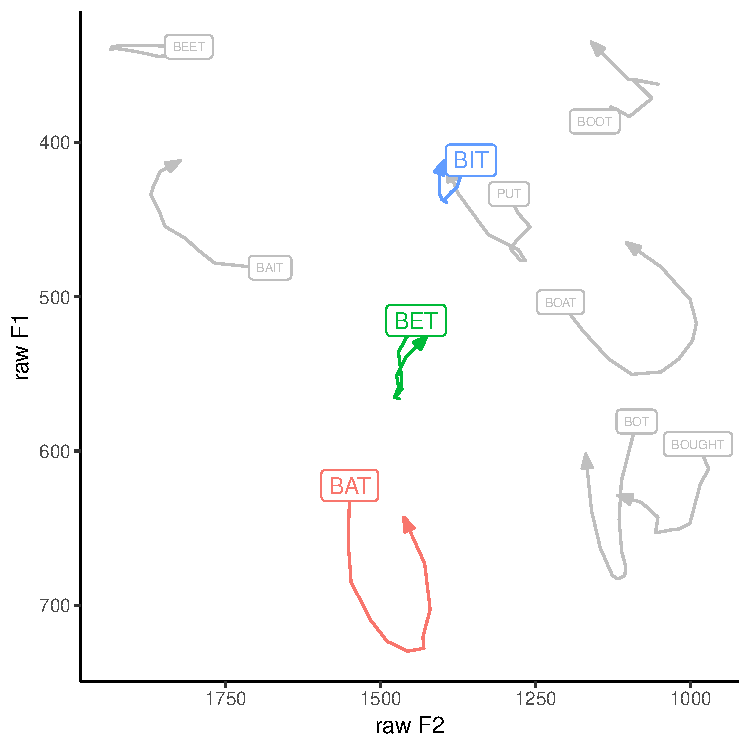
\includegraphics[width = \textwidth]{Figures/example_plots/15-Andrew_avg_traj.pdf}
        \caption{Andrew, who appreciates the Pacific Northwest, has more conservative vowels.}
        \label{fig:avg_traj_andrew}
    \end{subfigure}
    \hspace{\fill}
    \begin{subfigure}[t]{2.925in}
        \centering
        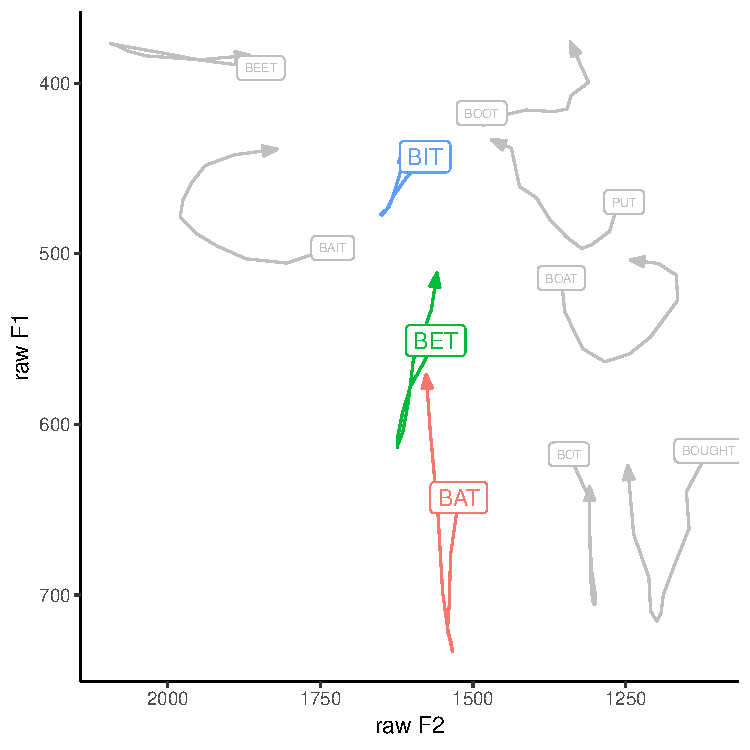
\includegraphics[width = \textwidth]{Figures/example_plots/47-Sean_avg_traj.pdf}
        \caption{Sean is more aligned to Portland and has more innovative variants.}
        \label{fig:avg_traj_sean2}
    \end{subfigure}
    \hspace{\fill}
    \caption{Average trajectories (in unnormalized Hz) for Millennial men who both go to Portland often and play in punk rock bands.}
    \label{fig:andrew_and_sean}
\end{figure*}


This affinity towards Portland, which was not found in the older generation, may be one reason why these Elsewhere Shift may be spreading into Cowlitz County, particularly in the younger speakers. The older generation had little reason to leave their community very often because it was relatively self-contained. This implies then that they were a somewhat insular community, and were not exposed to the linguistic changes occurring in nearby regions. On the other hand, the younger people are looking for any reason to leave town---and many have. Those who stayed crave some sort of entertainment or something new because they find Longview, Kelso, and Cowlitz County generally boring. Naturally, they would have been drawn to Portland because it was the nearest urban area, but it appears that they are especially fond of it because of its culture. It satisfies some need for entertainment that their ``boring'' city cannot. As a result, they go there much more often than the older generations do, and are therefore exposed to new and innovative linguistic variants found there.


So how does Seattle fit into this mix? The positive feelings towards Portland may or may not be accompanied with equally positive feelings towards Seattle. A few people like Megan liked both cities.
\begin{num_quote}
    I love Portland. And every time- every so often on TV shows you can tell when something is filmed in Portland, and I'm like, ``I love this show even more now!'' But it's the same with- with, um, with Seattle. I've always liked Seattle and had always wanted to live in Seattle, so it was nice to live in Seattle for that little bit of time. (Megan, 24, F)
    \label{quote:i_like_both}
\end{num_quote}
Many other interviewees shared Megan's feelings of wanting to see more of Seattle, but Megan was in the minority for liking Seattle as much as Portland, or even at all. There was not an overt dislike for the city, but there were some negative feelings, sometimes because of unfamiliarity but other times because of too much familiarity.
\begin{num_quote}
    \textit{Have you noticed a difference in sort of the culture between Seattle and Portland?}

    Seattle, I feel like every time I go there it's straight up ninety percent tourists. Yeah, and, uh. it's, well, y'know, but then again I'm going up there to visit the sites and going to Mariner games, y'know. I- it's not like I'm staying weeks up there or anything. So, um, but yeah. Yeah, I like Portland more than Seattle. I'll go on- yeah, I'll go on record saying that. (Andrew, 32, M)
    \label{quote:seattle_tourists}
\end{num_quote}
\begin{num_quote}
    I don't know, I feel like once you've seen Seattle you've kinda just seen it. Like Pikes Place Market, I've been there a dozen times. It's the same thing. Or Gas Works where there's like a view. Been there. I don't know, I feel like- it's just like- Portland it's always fun. Like there's just weird people you can watch all the time and like find weird random hole-in-the-wall places to eat, but… There's people at [my university in the Northeast] who are like, ``Oh my god, you're by- you're from by Portland!'' And like, ``Yeah, like I go there pretty often.'' They're like, ``Oh my god, I've seen \textit{Portlandia}. I just wanna go there so bad!'' I'm like, ``Well, I mean, it's like it- I mean, it's not exactly like it, so don't give your hopes up in that way.'' But it's pretty cool. (Kayla, 19, F)
    \label{quote:its_the_same_thing}
\end{num_quote}
So to these people, Seattle is ``just another'' big city---too big in fact---with little character to make it stand out. It appears then that these people's dislike for Seattle is not simply because it is farther away. Instead, they likely see it as just not as interesting as Portland:
\begin{num_quote}
    I usually go to Portland a lot cuz it's like thirty, forty minutes away, um, yeah… I mean like, comparing Portland and Seattle, Seattle's like really urban and more like- it's a big city. Portland's more- kinda like hipster. Manbuns, beards, coffee, biking. And Seattle, it's like… I don't know. It's bigger, yeah. (Hannah, 19, F)
    \label{quote:seattle_is_far}
\end{num_quote}
Because they do not get a chance to go there very often, they tend to go to the sites with many other tourists. Since those areas are often big and crowded, these smaller-town residents appear to prefer staying away from such urban areas. In essence, Seattle is seen as big and boring. Meanwhile, Portland is viewed as more of a smaller town with hole-in-the-wall restaurants and hipster culture, which make it familiar and interesting.

Summarizing these comments, there are clear patterns in how much people like Seattle and Portland, some of which are age-graded. For Seattle, people usually had less to say, primarily because the city is farther away and few of these speakers went there frequently. When they do go, it is mostly for tourism or to attend large events. In general, Seattle too is distant, too urban, and---in the eyes of these participants---too generic to have much of in impact on Cowlitz County. As for Portland, older residents of Cowlitz County are not particularly fond of it. While they do go there more often than Seattle, they do so out of necessity or for special occasions. None of them expressed an overt dislike for its culture, but no one had positive things to say about it either. The younger generation on the other hand appears to visit Portland far more frequently and for entertainment and leisure activities rather than necessity, such as to attend concerts, dining, shopping, or just simply to walk around. They acknowledge and enjoy the ``Keep Portland Weird'' slogan and describe the Portland as an interesting and hipster city with a small-town charm and full of different people and cultures. To summarize, these people were mostly apathetic towards Seattle and few of them went there with any regularity; older people did not like Portland, but younger people did.

These views of Seattle and Portland, particularly with the change towards the positive in the younger generation, help explain the linguistic patterns found in Cowlitz County. As the culture of Longview changed in the late 1970s and early 1980s from having relative prosperity and plenty of entertainment to having high unemployment and nothing to do, the younger people turned to their nearest urban neighbor. This increased communication with Portland likely exposed Millennial-aged Cowlitz County residents to new speech patterns, like innovative variants of the Elsewhere Shift, that their parents and grandparents did not hear as often. Because Portland is ``cool,'' these variants became associated with all things Portland---or at the very least, positive attributes that Cowlitz County lacked. It is out of the scope of this study to do an in-depth analysis of what these variants index, both for the speaker and listener in Cowlitz County, and to establish an indexical field of the shifted vowels, but future work may be able to address these social meanings.



\section{The timber industry}

So far, \S\ref{sec:then_and_now}, I established that younger people orient themselves away from Cowlitz County and in \S\ref{sec:portland_vs_seattle}, I showed that they instead orient themselves towards Portland. The question that remains is: why did the change even happen in the first place?

In \S\ref{sec:rise_and_fall}, I described the rise and fall of the timber industry in Cowlitz County. The mills still exist today, but they are not a central, integral part of the culture of Cowlitz County as they once were. I pointed out that the pivotal year was 1977. This was the year that the mills peaked at 12,210 employees in the region. Because of changes in the industry involving oversea prices and competition, mill workers all across the Pacific Northwest went on strike and many lost their jobs (or quit). This was exacerbated by Mount St. Helens' eruption in 1980 and the national recession in the early 1980s. Cowlitz County never quite recovered from where it once was.

This was around the start of when the Millennial generation is defined. All the older people grew up in a community where high-paying jobs at the mills were easy to get and there was no reason to leave the relatively prosperous area. However, the Millennials grew up in a different Cowlitz County. There were numerous financial struggles and jobs at the mills were no longer guaranteed (and often required a college degree). It makes sense now why they shifted their orientation away from their hometown---to find a job they had to.

% \begin{figure*}[tb!]
%     \centering
%     \includegraphics[width = 6.5in]{Figures/other_figures/changing_community.pdf}
%     \caption{Vowel shifts coincide with local community changes.}
%     \label{fig:changing_community}
% \end{figure*}

In the previous three chapters, I described numerous linguistic changes that the Millennials participated in. While the shifting of \bat and \bet appear to be independent of these changes, Millennials retracted \bit more than the previous generations, completing the shift. The biggest differences were in the prenasal vowels: Millennial women reversed the \ban lowering that the Generation X speakers did and now have a drastic prenasal split in \trap. Even \ben and \bin, while not as drastic of a change, are more monophthongal and have a ``pointier'' trajectory than the older speakers. Similarly, \bang and \bing were higher among the younger speakers. The majority of these changes were strongest in the women of Cowlitz County and they all are in the direction of changes documented in California and, by extension, Portland. Figure \ref{fig:changing_community} illustrates how these changes in the community line up with vowel shifts.

In addition to adopting innovative variants from areas to the south, the younger speakers suddenly abandoned conservative forms found in the North. As mentioned previously, \bag-raising is a feature that is associated with Washington and the Pacific Northwest. While it can be found in older speakers in Oregon, it is far more frequent and robust even in younger Seattleites, as well as in people from British Columbia and other parts of Canada. In Cowlitz County and other areas of the Pacific Northwest, a raised \bag indexes appreciation for traditional Pacific Northwest industries \citep{swan_2018_CWSL, stanley_2018_pwpl}. As younger people orient themselves away from the Pacific Northwest, it follows that they would avoid using linguistic variants that are associated with the region.

Therefore, it appears that much of this cultural shift can trace its roots to the changing timber industry in Cowlitz County. In the late 1970s and early 1980s, the economic downturn led to negative feelings towards the area, creating a social divide between the young and the old. The young people then oriented themselves towards Portland as their source of entertainment, culture, and, as shown in this section, speech variants.





\section{The northward spread of the Elsewhere Shift}

These results are among the first to show that the Elsewhere Shift has crossed the Columbia River northward into Washington State. Because the Elsewhere Shift is not present in Seattle or other parts of Eastern Washington \citep{wassink_2016_pads}, it is unlikely that the shift in Cowlitz County is a result of influence from Canada. Instead, in light of the increasingly positive views that speakers in this community have towards Portland, there is every reason to believe that the spread of the Elsewhere Shift into Cowlitz County was indeed northward from Portland.

\citeauthor{fridland_etal_2016_pads} suggest that the Elsewhere Shift, or at least \bat retraction, is ``an incoming new norm for the West Coast'' \citeyearpar[161]{fridland_etal_2016_pads}. Disregarding Canadian instantiation of the shift for a moment, it seems likely that the Elsewhere Shift originated in California, given the early reports of \citet{hinton_etal_1987}. As it moved its way up the Pacific Coast, it spread to the Willammette Valley and eventually to Portland. \citeauthor{mclarty_etal_2016} suggest that speakers born between the two World Wars were perhaps the first to adopt the shift in Oregon \citeyearpar[153]{mclarty_etal_2016}. The current study suggests that it has moved past the Washington border and at least into Cowlitz County. It is unclear when the shift first began in this community because the rate of change for these variables appears roughly constant. It is difficult to say whether the oldest generation has shifted vowels because of the lack of comparable non-shifted data, but certainly by the 1960s, speakers in Cowlitz County were adopting more innovative variants than their parents did, which has continued at least through the youngest adults today. Exactly how Canada fits into this is unclear at the moment, and this dataset does not help reconcile the similarities between the two regions. But it does offer evidence for the northward direction of the change. Furthermore, because these changes happened long before the 1970s, it appears that the Elsewhere Shift is not necessarily related to the timber industry and cultural shift in Cowlitz County, though it may have quickened the adoption of innovative variants.

Because the Elsewhere Shift is not present in Seattle or other parts of Eastern Washington \citep{wassink_2016_pads}, documenting its progress in Cowlitz County already noteworthy and makes this community stand out among other areas in the state. It also shows that Washington is not a uniform dialect area. Whether the patterns observed in Cowlitz County can be found in other areas of southwest Washington is unknown. Additional work in nearby communities would shed some light on the spread of the Elsewhere Shift up the Pacific Coast.


\section{Conclusions}

This chapter has provided evidence to suggest that Millennials in Cowlitz County orient themselves away from their community and towards Portland. There is a clear divide between older and younger people with respect to their views of Cowlitz County, which is backed up by comments from numerous speakers in this sample. This timing of these cultural shift correlates with many of the changes in the speech of Cowlitz County residents (particularly the prenasal allophones of the front lax vowels); correlation is not causation, but similar patterns have been documented in other communities across the country. Nevertheless, because the low back merger and subsequent shifting of \bat and \ben occurred before this cultural divide, I suggest that the Elsewhere Shift has been present in Cowlitz County just as long as it has been in Oregon, which may not be much later than California or Canada.
